%% LaTeX Template for ISIT 2019
%%
%% by Stefan M. Moser, October 2017
%% 
%% derived from bare_conf.tex, V1.4a, 2014/09/17, by Michael Shell
%% for use with IEEEtran.cls version 1.8b or later
%%
%% Support sites for IEEEtran.cls:
%%
%% http://www.michaelshell.org/tex/ieeetran/
%% http://moser-isi.ethz.ch/manuals.html#eqlatex
%% http://www.ctan.org/tex-archive/macros/latex/contrib/IEEEtran/
%%

\documentclass[conference,letterpaper]{IEEEtran}

%% depending on your installation, you may wish to adjust the top margin:
\addtolength{\topmargin}{9mm}

%%%%%%
%% Packages:
%% Some useful packages (and compatibility issues with the IEEE format)
%% are pointed out at the very end of this template source file (they are 
%% taken verbatim out of bare_conf.tex by Michael Shell).
%
% *** Do not adjust lengths that control margins, column widths, etc. ***
% *** Do not use packages that alter fonts (such as pslatex).         ***
%
\usepackage[utf8]{inputenc} 
\usepackage[T1]{fontenc}
\usepackage{url}
\usepackage{ifthen}
\usepackage{cite}
\usepackage[cmex10]{amsmath} % Use the [cmex10] option to ensure complicance
                             % with IEEE Xplore (see bare_conf.tex)

%% Please note that the amsthm package must not be loaded with
%% IEEEtran.cls because IEEEtran provides its own versions of
%% theorems. Also note that IEEEXplore does not accepts submissions
%% with hyperlinks, i.e., hyperref cannot be used.
\usepackage{graphicx}

%% Macros
\def\trainingset{\{x_i,y_i\}_{i=0}^{N-1}}
\def\pnmlSingle{\max_{\theta} P_\theta (y_N|x_N, z^N)}

\interdisplaylinepenalty=2500 % As explained in bare_conf.tex


%%%%%%
% correct bad hyphenation here
\hyphenation{op-tical net-works semi-conduc-tor}

% ------------------------------------------------------------
\begin{document}
\title{Predictive Normalize Likelihood for Least Squares: Toward Better Understanding of Generalization} 

%%% Several authors with up to three affiliations:
\author{%
  \IEEEauthorblockN{Koby Bibas}
  \IEEEauthorblockA{School of Electrical Engineering\\
                    Tel Aviv University\\
                    Email: kobybibas@gmail.com}
  \and
  \IEEEauthorblockN{Meir Feder}
  \IEEEauthorblockA{School of Electrical Engineering\\
                    Tel Aviv University\\ 
                    Email: meir@eng.tau.ac.il}
}


%%% Many authors with many affiliations:
% \author{%
%   \IEEEauthorblockN{Albus Dumbledore\IEEEauthorrefmark{1},
%                     Olympe Maxime\IEEEauthorrefmark{2},
%                     Stefan M.~Moser\IEEEauthorrefmark{3}\IEEEauthorrefmark{4},
%                     and Harry Potter\IEEEauthorrefmark{1}}
%   \IEEEauthorblockA{\IEEEauthorrefmark{1}%
%                     Hogwarts School of Witchcraft and Wizardry,
%                     1714 Hogsmeade, Scotland,
%                     \{dumbledore, potter\}@hogwarts.edu}
%   \IEEEauthorblockA{\IEEEauthorrefmark{2}%
%                     Beauxbatons Academy of Magic,
%                     1290 Pyrénées, France,
%                     maxime@beauxbatons.edu}
%   \IEEEauthorblockA{\IEEEauthorrefmark{3}%
%                     ETH Zürich, ISI (D-ITET), ETH Zentrum, 
%                     CH-8092 Zürich, Switzerland,
%                     moser@isi.ee.ethz.ch}
%   \IEEEauthorblockA{\IEEEauthorrefmark{4}%
%                     National Chiao Tung University (NCTU), 
%                     Hsinchu, Taiwan,
%                     moser@isi.ee.ethz.ch}
% }


\maketitle

%%%%%%
%% Abstract: 
%% If your paper is eligible for the student paper award, please add
%% the comment "THIS PAPER IS ELIGIBLE FOR THE STUDENT PAPER
%% AWARD." as a first line in the abstract. 
%% For the final version of the accepted paper, please do not forget
%% to remove this comment!
%%
\begin{abstract}
This work deals with universal prediction under the individual setting in the regression problem. 
Given a training set and a hypothesis class, our goal is to predict the label of a test sample. 
Since the data and labels are individual, the objective of universal predictor is to be as good as the best predictor from a given hypothesis class. 
We use the Predictive Normalized Maximum Likelihood (PNML) scheme, a robust learning solution that also provides an indication for the learnability of a specific test sample based on the training set and hypothesis class. 
We present an analytic solution for the regression problem with least squares hypothesis class and perform an evaluation of the learnable space. 
We demonstrate our results with a simulation of fitting a polynomial curve to a data with various regularization terms and polynomial degrees.
\end{abstract}

%%%%%%%%%%%%%%%%%%%%%%%%%%%%%%%%%%%%%%%%%%%%%%%%%%%%%%%%%%%%%%%%%%%%%%%%%%%%%%%%

\section{Introduction} \label{Introduction}
In machine learning, the most common tasks are classification and regression. In classification, given training set which consist N pairs $z^N=\{(x_i, y_i)\}_{i=0}^{N-1}$, where $x \in \mathcal{X}$ is the data and $y \in \mathcal{Y}$ are the labels for which $\mathcal{Y}$ is a finite set, the goal is to predict the label $y_N$ of unseen data $x_N$. 
The regression task settings are the same as the classification except that the label space $\mathcal{Y}$ is infinite and continuous.
In order to evaluate the performance of some predictor $q$ on a test sample $(x_N, y_N)$, a loss function  $\mathcal{L}$ is required. Using the framework of the information theory field, we consider the log-loss as the loss function
\begin{equation}
\mathcal{L}(q,x_N,y_N) = -P(y_N|x_N)\log {q(y_N|x_N}),
\end{equation}
where $P(y_N|x_N)$ is the true probability assignment.
The best predictor is one who has the minimal loss for all test samples.

The main settings of the way the pairs $\{x,y\}$ are generated are the stochastic, the Probably Approximately Correct (PAC) and individual. 
In the stochastic setting the data and labels are assumed to be generated from a probabilistic source, i.e. there is probabilistic assignment $P_\theta(y|x)$ from a set of hypothesis class $\theta \in \Theta$ and our goal is to find it. 

The concept of PAC was established in  \cite{valiant1984theory}.
In this setting, the data samples assumed to be generated independently from some source $P(x,y)=P(x)P(y|x)$, however, unlike the stochastic setting, $P(y|x)$ is not necessarily a member of the hypothesis class.
The purpose in this setting is to design an algorithm that attains, with very high probability over the possible training sets, a loss which is almost the same as the loss of the best hypothesis in the class. 

In this paper, we consider the scenario of the individual setting. 
In the individual setting the assumption that the data and labels were created by probabilistic mechanism is no longer valid and finding an assignment of y given x is therefore impossible. 
The goal now becomes to be as good as possible as a learner who has information about the training set along with the label of the test sample. 
We call this kind of learner a Genie \cite{feder1992universal}. The Genie has some constraints: it is restricted to be a member of a hypothesis class $\{P_\theta(y_N|x_N,y_N,z^N)\ , \ \theta \in \Theta \}$.  
In addition, it has no knowledge about which of the sample it is going to be tested on. 
The log-loss difference between our learner and the Genie is known as the regret
\begin{multline} \label{eq:genie_regret}
R(\theta, q, x_N, z^N) = \\ \sum_{y \in \mathcal{Y}} P_\theta(y_N|x_N,y_N,z^N) log \frac{P_\theta(y_N|x_N,y_N,z^N)}{q_(y_N|x_N, z^N)}.
\end{multline}

% ERM
The most common approach of generating a leaner is the Empirical Risk Minimization (ERM) \cite{vapnik1992principles}. 
Given a training set and hypothesis class $\{P_\theta(y|x),\ \theta \in \mathcal{\theta}\}$, a predictor that minimizes the training set error is chosen
\begin{equation}
Q(y|x) = \min_\theta \frac{1}{N}\sum_{i=0}^{N-1}  l(y_i,P_\theta(y_i|x_i)).
\end{equation}
The underline assumptions of the ERM approach are that data is generates as in the stochastic setting and that the training samples are generated independently.

% PNML
In this paper we use the Predictive Normalized Likelihood (PNML). The PNML is the solution of the min-max problem of equation \ref{eq:genie_regret} \cite{shtar1987universal}
\begin{equation} \label{eq:minmax_prob}
Q_{\textit{PNML}}(\cdot|x_N,z^N) = \underset{q}{\textit{argmin }}\underset{y_N}{\textit{max }} R(\theta, q, x_N, z^N)
\end{equation}
and the solution is 
\begin{equation} \label{eq:pnml}
Q_{PNML}(y_N|x_N,z^N)=\frac{\pnmlSingle}{\sum_{y\in \mathcal{Y}} \pnmlSingle}.
\end{equation}
In order to obtain the PNML predictor the following procedure is executed:  assuming the label of the test data is known, fit a learner to it and predict the assumed label by it. 
Repeat the process for all possible label. 
In the end, normalize the probabilities from each label and return the PNML predictor.
The regret of the PNML predictor is its normalization factor
\begin{equation} \label{eq:pnml_regret}
R(Q_{\textit{PNML}}, x_N, z^N) = \log \left\{ \sum_{y\in \mathcal{Y}} \pnmlSingle \right\}.
\end{equation}

% Least Squares
This paper deals with the least squares model family, which is a standard approach in regression analysis \cite{lawson1995solving}. 
In this approach, the overall solution minimizes the sum of the squares of the residuals. The common assumption is that the number of training samples needs to be much higher than the number of features in order to be able to generalize \cite{james2013introduction}.
Recently, the success of Deep Neural Network (DNN) in which the number of learnable parameters is in several order of magnitudes greater than the size of the feature space requires rethinking that assumption.

In summary, this paper provides two main contributions.
First, we present an analytic solution of the PNML predictor for the least squares hypothesis class. Second, we introduce the learnable space- the space from which if the test data is lied in, a relabel prediction can be made by the PNML predictor. We show that it is indeed possible to learn even when the number of training samples is smaller than the number of features.

The paper outline is as follows.
Section \ref{sec:related_works} presents the related. Section \ref{sec:formal_problem_def} introduces the setting and the goal of the regression problem. In section \ref{sec:PNML_eval} the evaluation of the PNML is presented and analyzed. In depth evaluation of the learnable space is shown in section \ref{sec:learnable_space}. The simulation of the PNML and its regret on estimating polynomial coefficients is shown in section \ref{sec:simulation} and the conclusion and future work is in section \ref{sec:conclusion}.

\section{Related Works} \label{sec:related_works}
We now provide a brief survey of work in the areas of universal prediction, model generalization and least squares predictions.

\textbf{Universal Prediction.}
The universal predictor is one that does not depend on the unknown underlying model and yet performs essentially as well as if the model were known in advance.
Many works were done in the universal predictions field under a different setting.
\cite{feder1992universal} presents a comprehensive survey of the universal prediction field under various settings: stochastic settings, individual settings and variety of loss functions. 
\cite{shtar1987universal} showed the min-max solution It is similar to the previous Normalized Maximum Likelihood, which is the solution in the context of on-line prediction of a sequence.  
\cite{Fogel2017} proposes a min-max universal learning solution that minimizes the worst case log-loss regret in the case of online learning.
The PNML scheme which solves the min-max problem from equation \ref{eq:minmax_prob} for batch learning in the individual settings is introduced in \cite{Fogel2018}.

\textbf{Model Generalization.} 
Understating the model generalization capabilities is considered fundamental problem in machine learning  \cite{vapnik2013nature}. 
The common approach is to use the VC Dimension for the upper bound on the test error.
For DNN, the VC dimension is linear with the number of parameters \cite{sontag1998vc}, however, recent empirical evidence demonstrates that they have state of the art performance which implies the bound is too loose.

\textbf{Least Squares}
The least squares algorithm is widely used due to 2 primary reasons: robust performance and simplicity of implementation.
Recursive least squares is an efficient online method for finding linear predictors minimizing the mean squared error over the training data \cite{hayes19969}.
So far the least squares for prediction was used in the ERM approach and in Bayesian linear regression \cite{fornalski2015applications}. For the best of our knowledge, there isn't work which use it as hypothesis class for the PNML scheme as we do.

\section{Formal Problem Definition} \label{sec:formal_problem_def}
Given N pairs of data and labels $\{x_i, y_i\}_{i=0}^{N-1}$ where $x_i \in R^M, y\in R$ are deterministic. Our model takes the form:
\begin{equation}
\begin{split}
y_0&=x_0^T \theta + e_0 \\
y_1&=x_1^T \theta + e_1 \\
   &\ \vdots \\
y_{N-1}&=x_{N-1}^T \theta + e_{N-1} \\
\end{split}
\end{equation}
where $\theta \in R^M$ are the learnable parameters and $e \in R$ is white Gaussian noise with variance of $\sigma$. 
Our goal is to predict $y_N$ based on a new data sample $x_N$:
\begin{equation}
y_N = x_N^T \theta + e_N.
\end{equation}
In this case $y_N$ has normal distribution that depends on the learnable parameters $\theta$ 
\begin{equation}
P_{\theta}(y_N) 
=\frac{1}{\sqrt[]{2\pi\sigma^2}}exp\left\{-\frac{1}{2\sigma^2}\big(y_N- x_N^T\theta \big)^2\right\}  \\
\end{equation}
We consider the $\theta$ to be a member of hypothesis class $\Theta$, which is the solution of the least squares problem
\begin{equation} \label{eq:ls_hypotheses_class}
\Theta := \left\{ \underset{\theta}{\textit{argmin }} \sum_{i=0}^{N-1} | x^T_i \theta - y |^2 \right\}.
\end{equation}
Denote $\gamma$ as the normalization factor of the PNML predictor
\begin{equation}
\Gamma=\int_R \max_{\theta \in \Theta} P_\theta(y_N|X^T)dy_N,   
\end{equation}
the PNML prediction of $y_N$ given the training set $\{x_i,y_i\}_{i=0}^{N-1}$ and the test sample $x_N$ is
\begin{equation} \label{eq:pnml_def}
Q_{\textit{PNML}}(y_N|x_N,z^N) = \frac{1}{\Gamma} \max_{\theta \in \Theta} P_\theta(y_N).
\end{equation}
The target is to find the analytic solution of equation \ref{eq:pnml_def} for least squares hypothesis class.

\section{PNML Evaluation} \label{sec:PNML_eval}
Using the notations $X \in R^{MxN+1}$ for a matrix which contains all the training set data along with the test sample, $y \in R^{N+1}$ to a vector which contains all the label and $e \in R^{N+1}$ for the noise vector
\begin{equation}
X = \begin{bmatrix} x_0 & x_1 & \dots & x_N \end{bmatrix}\ \ 
y = \begin{bmatrix} y_0 \\ y_1 \\ \vdots \\ y_N \end{bmatrix}\ \
e = \begin{bmatrix} e_0 \\ e_1 \\ \vdots \\ e_N  \end{bmatrix}.
\end{equation}
Assuming that the label of $x_N$ is given ($y_N$ is known), the optimal solution under the mean square error is the least squares estimator:
\begin{equation}
\theta ^*_N = (X^T X)^{-1} X y
\end{equation}
Rewrite it in the recursive least square formulation \cite{hayes19969}:
\begin{equation} \label{eq:rls_update}
\theta ^*_N = \theta^*_{N-1} - P_N x_N (y_N - \hat{y}_N)
\end{equation}
where $\hat{y}_N = x_N^T \theta ^*_{N-1}$ is the ERM predictions based on the samples $\{x_i, y_i\}_{i=0}^{N-1}$ and $P_N$ is the inverse covariance matrix of the data.
Without loss of generality, $\mu _{X} = 0$ and therefore the inverse covariance matrix becomes the inverse correlation matrix
\begin{equation}
P_N = (XX^T)^{-1}. 
\end{equation}
The probability distribution of our estimation of $y_N$ can be written as
\begin{equation}
\begin{split}
&P_{\theta_N ^*}(y_N) 
=\frac{1}{\sqrt[]{2\pi\sigma^2}}exp\left\{-\frac{1}{2\sigma^2}\big(y_N- x_N^T\theta ^*_N \big)^2\right\} = \\
& \qquad \frac{1}{\sqrt[]{2\pi\sigma^2}}exp\bigg\{-\frac{1}{2\sigma^2}\big(y_N - x_N^T \big(\theta^*_{N-1} + \\ 
& \qquad \qquad \qquad \qquad \qquad P_N x_N (y_N -\hat{y}_N) \big) \big)^2\bigg\} = \\
% =\frac{1}{\sqrt[]{2\pi\sigma^2}}
% exp\left\{-\frac{1}{2\sigma^2}\left((1-x_N^T P_N x_N)y_N-\hat{y}_N + x_N^T P_N x_N\hat{y}_N \right)^2\right\}  \\
% =\frac{1}{\sqrt[]{2\pi\sigma^2}}
% exp\left\{-\frac{1}{2\sigma^2}\left((1-x_N^T P_N x_N)y_N-(1 - x_N^T P_N x_N )\hat{y}_N \right)^2\right\}  \\
& \qquad \frac{1}{\sqrt[]{2\pi\sigma^2}}
exp\left\{-\frac{(1 - x_N^T P_N x_N )^2 }{2\sigma^2}\left(y_N-\hat{y}_N \right)^2\right\}.  \\
\end{split}
\end{equation}
Looking back to the PNML normalization factor from equation \ref{eq:pnml_def}
\begin{multline}
\Gamma = \int_R \max_{\theta} P_\theta(y_N|X^T)dy_N = \\
\int_{-\infty}^{\infty} \frac{1}{\sqrt[]{2\pi\sigma^2}}
\ exp\left\{-\frac{(1 - x_N^T P_N x_N )^2 }{2\sigma^2}
\left(y_N- \hat{y}_N \right)^2\right\} dy_N\\ 
=\frac{1}{1 - x_N^T P_N x_N } 
=\frac{1}{1 - x_N^T (XX^T)^{-1} x_N } \\
\end{multline}
Finally, given a new data sample $x_N$ the PNML of $y_N$ is:
\begin{multline}
Q_{PNML}(y_N | x_N, z^N) = \frac{1}{\Gamma}\max_{\theta}P_{\theta}(y_N) = \\
\frac{1 - x_N^T P_N x_N }{\sqrt[]{2\pi\sigma^2}}
exp\left\{-\frac{(1 - x_N^T P_N x_N )^2 }{2\sigma^2}\left(y_N-\hat{y}_N \right)^2\right\} \\
\end{multline}

We can also calculate the regret of the PNML. From equation \ref{eq:pnml_regret}, the regret is the log of the PNML normalization factor
\begin{equation} \label{eq:regret}
log(\Gamma) = \log\left(\frac{1}{1 - x_N^T (XX^T)^{-1} x_N } \right).
\end{equation}
The regret is associated with the uncertainty of the model prediction of the test sample. It can be seen that it depends on the hypothesis class (the least squares in this case) and on the data.

\section{PNML with Regularization} \label{sec:PNMLwithReg}
The previous section dealt with the least squares predictor hypothesis class. Here we show the evaluation in case of the least squares with Tikhonov regularization 
\begin{equation}
\mathcal{L}(z^N)= \sum_{i=0}^{N-1}|y_i-x_i^T \theta|^2 + \lambda ||\theta||_2^2
\end{equation}
where $\lambda$ is the regularization term.
The hypothesis class is therefore is changed to
\begin{equation} \label{eq:ls_reg_hypotheses_class}
\Theta := \left\{ \underset{\theta}{\textit{argmin }} \sum_{i=0}^{N-1} | x^T_i \theta - y |^2 + \lambda ||\theta||_2^2 \right\}.
\end{equation}
In this case the solution of the least squares predictor is
\begin{equation}
\theta ^*_N = (X^T X+ \lambda I)^{-1} X y
\end{equation}
Rewrite it in the recursive least square formulation 
\begin{equation}
\theta ^*_N=\theta^*_{N-1} - P_N x_N (y_N - \hat{y}_N)
\end{equation}
which is the same as Equation \ref{eq:rls_update}, however, in this case the inverse correlation matrix is 
\begin{equation}
P_N= (X^T X+ \lambda I)^{-1}.    
\end{equation}
The rest of the PNML evaluation stays the same and therefore the normalization factor becomes
\begin{equation}
\Gamma =\frac{1}{1 - x_N^T (XX^T+ \lambda I)^{-1} x_N } 
\end{equation}
and the predictor is 
\begin{multline} \label{eq:pnml_least_sqaures}
Q_{PNML}(y_N,x_N, z^N, \lambda)
=\frac{1 - x_N^T (XX^T + \lambda I)^{-1} x_N }{\sqrt[]{2\pi\sigma^2}} \\
\cdot exp\left\{-\frac{(1 - x_N^T (XX^T + \lambda I)^{-1} x_N )^2 }{2\sigma^2}\left(y_N- \hat{y}_N \right)^2\right\} \\
\end{multline}
The regret of least squares with Tikhonov regularization hypothesis class is
\begin{equation}
\log (\Gamma) = \log \left( \frac{1}{1 - x_N^T (XX^T + \lambda I)^{-1} x_N } \right)
\end{equation}
The regularization helps the inversion of the correlation matrix in the case of ill conditions. In the next section we derive the space in which that kind of regularization is needed.

\section{Learnable Space} \label{sec:learnable_space}
In order to understand for which test sample the trained model generalized well we need to evaluate the regret expression from equation \ref{eq:regret}. High regret means that our model is very far from the Genie and therefore we cannot trust its predictions. Low regret, on the other hand, means the model is as good as a Genie who has the knowledge about the label of the test sample.

Applying the singular value decomposition (SVD) on the training set $[x_0,x_1, \hdots, x_{N-1}] = U \Sigma V^T$ with $U\in R^{MxM}$, where M is the number of features ($x_N \in R^M$) and $\Sigma$ is rectangular diagonal matrix with diagonal values $\{\eta_i\}_{i=0}^{min(M,N)} \ $. The expression $x_N^T(XX^T)^{-1}x_N$ ca be rewritten as follows:
\begin{multline}
x_N^T(XX^T)^{-1}x_N = \\
x_N^T\left(\begin{bmatrix} U \Sigma V^T & x_N \end{bmatrix}
\begin{bmatrix}
V \Sigma^T U^T \\ x_N^T
\end{bmatrix}
\right)^{-1}x_N \\
=  x_N^T\left(U \Sigma \Sigma^T U^T + x_N x_N^T\right)^{-1}x_N.
\end{multline}
Using Sherman Morrison formula \cite{press2007section}, denote 
\begin{equation}
A=U \Sigma \Sigma^T U^T \ \ A^{-1}=U (\Sigma \Sigma^T)^{-1} U^T   
\end{equation}
Our expression get the following form:
\begin{equation}
x_N^T(XX^T)^{-1}x_N = 
x_N^T \left[ A^{-1} -  \frac{ A x_N x_N^T  A}{1 + x_N^T  A x_N} \right] x_N.
\end{equation}
Denote $\gamma = x_N^T  U (\Sigma \Sigma^T)^{-1} U^T x_N$, we can simplify the expression to:
\begin{equation}
x_N^T(XX^T)^{-1}x_N = \gamma - \frac{\gamma^2}{1+\gamma} = \frac{\gamma}{1+\gamma}.
\end{equation}
Plug in to the regret from equation \ref{eq:regret}:
\begin{equation}
\log \Gamma = \log \left( \frac{1}{1-\frac{\gamma}{1+\gamma}} \right)
=  \log \left( 1+\gamma \right).
\end{equation}
$\gamma$ can be expressed with the projection of $x_N$ on the correlation matrix of the training set:
\begin{multline}
\gamma = 
\begin{bmatrix}
x_N^T u_0 & \hdots & x_N^T u_M
\end{bmatrix}
\begin{bmatrix}
\frac{1}{\eta_0^2} & \hdots & 0 \\
0 & \hdots &  0 \\
\vdots & \vdots &  \vdots \\
0 & \hdots &  \frac{1}{\eta_m^2} \\
\end{bmatrix}
\begin{bmatrix}
u_0^T x_N \\ \vdots \\ u_m^T x_N
\end{bmatrix} \\
= \sum_{i=0}^M \left(\frac{u_i^T x_N}{\eta_i}\right)^2.
\end{multline}
The final regret expression is
\begin{equation}
\log \Gamma = \log \left(1 +  \sum_{i=0}^M \left(\frac{u_i^T x_N}{\eta_i}\right)^2 \right).
\end{equation}

$u_i^T x_N$ is the projection of $x_N$ on the i-th dimension of the correlation matrix of the training set. If the test sample $x_N$ lies mostly in the subspace spanned by the eigenvectors with large eigenvalues, then the model can generalize well for it. If the test sample is in the subspace where the eigenvalues are small (or zeros), the regret will be very large and we can deduce that the model prediction is now reliable.

\section{Simulation} \label{sec:simulation}
In this section a  simulation which shows the regret is presented.
We've chosen to focus on the problem of polynomial curve fitting. 
We show the differences in predictions and generalization capabilities between a variety of regularization terms and various polynomial degrees.

\subsection{Least Squares with Regularization} \label{sec:least_sqaures_with_reg}
We compare predictions of least squares hypothesis class with different regularization terms.
We generated 3 random points uniformly in the interval $t_i \in [-1, 1],\ i \in \{0,1,2\}$. We use these points as the training set. 
The points are shown in Figure \ref{fig:least_squares_with_reg} (top) as red dots. 
Assuming the data generated from 2 degree polynomial, we constructed X matrix as in section \ref{sec:formal_problem_def}:
\begin{equation}
X = 
\begin{bmatrix}
1 & 1 & 1 \\
t_0 & t_1 & t_2 \\
t_0^2 & t_1^2 & t_2^2 
\end{bmatrix}.
\end{equation}
We predict the values of all t values in the interval [-1,1] using equation \ref{eq:pnml_least_sqaures} with regularization terms $\lambda$ of 0, 0.1 and 1.0. 
It is shown in Figure \ref{fig:least_squares_with_reg} (top) that without regularization, the blue curve fits exactly to the data, and as increasing the regularization the curve becomes less steep and tends to fit less to the training data.

Figure \ref{fig:least_squares_with_reg} (bottom) shows the regret from equation \ref{eq:regret} of the 2 degree polynomial prediction of the same points $t_i$. 
The t values are marked in red on the x axis. 
We can see that around the training data the regret is very low in comparison to areas where training data don't exist. 
In addition, with regularization, the overall regret is lower and is greater than 0.5 only in the edges of the interval.
For all regularization terms, the regret values explode as moving away from the training data.

\begin{figure}[h] 
    \centering
    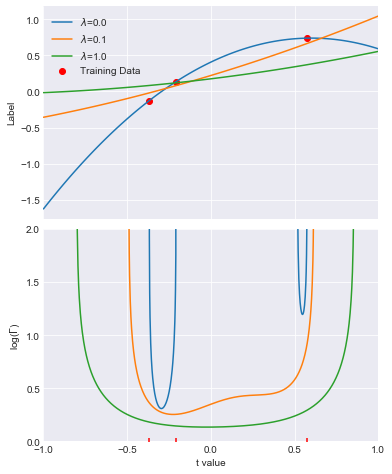
\includegraphics[width=\linewidth]{figures/least_sqaures_with_regularization.jpg}
    \caption{\textbf{Least squares predictor with variety of regularization terms.} (Top) The least squares estimator fitted to the training data (in red) with different values of regularization term. (Bottom) The regret of the PNML predictor from equation \ref{eq:regret} on the interval [-1,1]. The training data t values are marked in red on the x axis.}
    \label{fig:least_squares_with_reg}
\end{figure}

\subsection{Least Squares with different Polynomial Degree} \label{sec:least_sqaures_with_pol_deg}
We simulate a case of fitting polynomial curves with different polynomial degrees. We again generated 3 random points uniformly in the interval $t_i \in [-1, 1],\ i \in \{0,1,2\}$.
We constructed X matrix based on the polynomial degree:
\begin{equation}
X = 
\begin{bmatrix}
1 & 1 & 1 \\
t_0 & t_1 & t_2 \\
\vdots \\
t_0^{\textit{Poly Deg}} & t_1^{\textit{Poly Deg}} & t_2^{\textit{Poly Deg}} 
\end{bmatrix}.
\end{equation}
Figure \ref{fig:least_squares_with_poly} (top) shows the predicted label for every t value in the interval [-1,1] for the different polynomial degrees. The training set is shown as red dots in this figure. 
For 3 degree polynomial, the number of features in greater than the size of the training set, however, the prediction in the area of the training set is similar to the prediction of 2 degree polynomial.
Figure \ref{fig:least_squares_with_poly} (bottom) shows the regret of the 3 PNML predictors. All of the predictors have regrets values that explode as drifting away from the training data, however, within t values of 0 and 0.6, the regret is relatively small and it seems that the prediction is indeed reliable in there.






\begin{figure}[h]
    \centering
    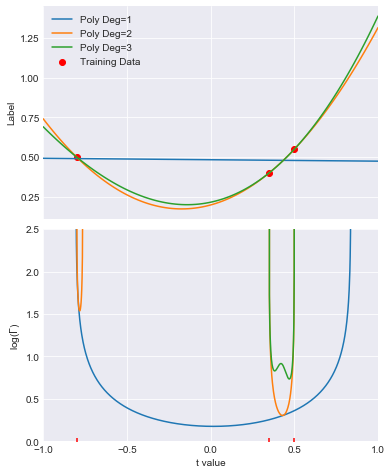
\includegraphics[width=0.98\linewidth]{figures/least_sqaures_with_poly_degree.jpg}
    \caption{\textbf{Least squares predictor with different polynomial degree.} (Top) PNML least squares predictions with different polynomial degrees. (Bottom) The regret of the PNML predictors from equation \ref{eq:regret} on the interval [-1,1]. The training data t values are marked in red on the x axis.}
    \label{fig:least_squares_with_poly}
\end{figure}


\section{Conclusions} \label{sec:conclusion}

In this paper, we have shown an analytic solution for the PNML prediction scheme under the least squares hypothesis class. The mean of that PNML prediction solution is ERM solution, however, using the PNML, training set based uncertainty measure is obtained. In addition, we analyzed the learnable space: the subspace spanned by the eigenvectors with large eigenvalues. If a test sample lies within that space, then the model can generalize well for it. 
In addition, we've shown a simulation of least squares prediction with different regularization terms and polynomial degrees the corresponding regret for each one. 

This work suggests a number of potential directions
for future work. These include: (1) evaluate the PNML predictors for more hypothesis classes. (2) Obtain the learnable space under the PAC and Stochastic setting.

\newpage

%%%%%%
%% To balance the columns at the last page of the paper use this
%% command:
%%
%\enlargethispage{-1.2cm} 
%%
%% If the balancing should occur in the middle of the references, use
%% the following trigger:
%%
% \IEEEtriggeratref{3}
%%
%% which triggers a \newpage (i.e., new column) just before the given
%% reference number. Note that you need to adapt this if you modify
%% the paper.  The "triggered" command can be changed if desired:
%%
%\IEEEtriggercmd{\enlargethispage{-20cm}}
%%
%%%%%%


%%%%%%
%% References:
%% We recommend the usage of BibTeX:
%%
%\bibliographystyle{IEEEtran}
%\bibliography{definitions,bibliofile}
%%
%% where we here have assume the existence of the files
%% definitions.bib and bibliofile.bib.
%% BibTeX documentation can be obtained at:
%% http://www.ctan.org/tex-archive/biblio/bibtex/contrib/doc/
%%%%%%


%% Or you use manual references (pay attention to consistency and the
%% formatting style!):
\bibliographystyle{IEEEtran}
\bibliography{refrences.bib}



\end{document}


%%%%%%
%% Some comments about useful packages
%% (extract from bare_conf.tex by Michael Shell)
%%

% *** MISC UTILITY PACKAGES ***
%
%\usepackage{ifpdf}
% Heiko Oberdiek's ifpdf.sty is very useful if you need conditional
% compilation based on whether the output is pdf or dvi.
% usage:
% \ifpdf
%   % pdf code
% \else
%   % dvi code
% \fi
% The latest version of ifpdf.sty can be obtained from:
% http://www.ctan.org/pkg/ifpdf
% Also, note that IEEEtran.cls V1.7 and later provides a builtin
% \ifCLASSINFOpdf conditional that works the same way.
% When switching from latex to pdflatex and vice-versa, the compiler may
% have to be run twice to clear warning/error messages.


% *** CITATION PACKAGES ***
%
%\usepackage{cite}
% cite.sty was written by Donald Arseneau
% V1.6 and later of IEEEtran pre-defines the format of the cite.sty package
% \cite{} output to follow that of the IEEE. Loading the cite package will
% result in citation numbers being automatically sorted and properly
% "compressed/ranged". e.g., [1], [9], [2], [7], [5], [6] without using
% cite.sty will become [1], [2], [5]--[7], [9] using cite.sty. cite.sty's
% \cite will automatically add leading space, if needed. Use cite.sty's
% noadjust option (cite.sty V3.8 and later) if you want to turn this off
% such as if a citation ever needs to be enclosed in parenthesis.
% cite.sty is already installed on most LaTeX systems. Be sure and use
% version 5.0 (2009-03-20) and later if using hyperref.sty.
% The latest version can be obtained at:
% http://www.ctan.org/pkg/cite
% The documentation is contained in the cite.sty file itself.


% *** GRAPHICS RELATED PACKAGES ***
%
\ifCLASSINFOpdf
  % \usepackage[pdftex]{graphicx}
  % declare the path(s) where your graphic files are
  % \graphicspath{{../pdf/}{../jpeg/}}
  % and their extensions so you won't have to specify these with
  % every instance of \includegraphics
  % \DeclareGraphicsExtensions{.pdf,.jpeg,.png}
\else
  % or other class option (dvipsone, dvipdf, if not using dvips). graphicx
  % will default to the driver specified in the system graphics.cfg if no
  % driver is specified.
  % \usepackage[dvips]{graphicx}
  % declare the path(s) where your graphic files are
  % \graphicspath{{../eps/}}
  % and their extensions so you won't have to specify these with
  % every instance of \includegraphics
  % \DeclareGraphicsExtensions{.eps}
\fi
% graphicx was written by David Carlisle and Sebastian Rahtz. It is
% required if you want graphics, photos, etc. graphicx.sty is already
% installed on most LaTeX systems. The latest version and documentation
% can be obtained at: 
% http://www.ctan.org/pkg/graphicx
% Another good source of documentation is "Using Imported Graphics in
% LaTeX2e" by Keith Reckdahl which can be found at:
% http://www.ctan.org/pkg/epslatex
%
% latex, and pdflatex in dvi mode, support graphics in encapsulated
% postscript (.eps) format. pdflatex in pdf mode supports graphics
% in .pdf, .jpeg, .png and .mps (metapost) formats. Users should ensure
% that all non-photo figures use a vector format (.eps, .pdf, .mps) and
% not a bitmapped formats (.jpeg, .png). The IEEE frowns on bitmapped formats
% which can result in "jaggedy"/blurry rendering of lines and letters as
% well as large increases in file sizes.
%
% You can find documentation about the pdfTeX application at:
% http://www.tug.org/applications/pdftex


% *** MATH PACKAGES ***
%
%\usepackage{amsmath}
% A popular package from the American Mathematical Society that provides
% many useful and powerful commands for dealing with mathematics.
%
% Note that the amsmath package sets \interdisplaylinepenalty to 10000
% thus preventing page breaks from occurring within multiline equations. Use:
%\interdisplaylinepenalty=2500
% after loading amsmath to restore such page breaks as IEEEtran.cls normally
% does. amsmath.sty is already installed on most LaTeX systems. The latest
% version and documentation can be obtained at:
% http://www.ctan.org/pkg/amsmath


% *** SPECIALIZED LIST PACKAGES ***
%
%\usepackage{algorithmic}
% algorithmic.sty was written by Peter Williams and Rogerio Brito.
% This package provides an algorithmic environment fo describing algorithms.
% You can use the algorithmic environment in-text or within a figure
% environment to provide for a floating algorithm. Do NOT use the algorithm
% floating environment provided by algorithm.sty (by the same authors) or
% algorithm2e.sty (by Christophe Fiorio) as the IEEE does not use dedicated
% algorithm float types and packages that provide these will not provide
% correct IEEE style captions. The latest version and documentation of
% algorithmic.sty can be obtained at:
% http://www.ctan.org/pkg/algorithms
% Also of interest may be the (relatively newer and more customizable)
% algorithmicx.sty package by Szasz Janos:
% http://www.ctan.org/pkg/algorithmicx


% *** ALIGNMENT PACKAGES ***
%
%\usepackage{array}
% Frank Mittelbach's and David Carlisle's array.sty patches and improves
% the standard LaTeX2e array and tabular environments to provide better
% appearance and additional user controls. As the default LaTeX2e table
% generation code is lacking to the point of almost being broken with
% respect to the quality of the end results, all users are strongly
% advised to use an enhanced (at the very least that provided by array.sty)
% set of table tools. array.sty is already installed on most systems. The
% latest version and documentation can be obtained at:
% http://www.ctan.org/pkg/array

% IEEEtran contains the IEEEeqnarray family of commands that can be used to
% generate multiline equations as well as matrices, tables, etc., of high
% quality.


% *** SUBFIGURE PACKAGES ***
%\ifCLASSOPTIONcompsoc
%  \usepackage[caption=false,font=normalsize,labelfont=sf,textfont=sf]{subfig}
%\else
%  \usepackage[caption=false,font=footnotesize]{subfig}
%\fi
% subfig.sty, written by Steven Douglas Cochran, is the modern replacement
% for subfigure.sty, the latter of which is no longer maintained and is
% incompatible with some LaTeX packages including fixltx2e. However,
% subfig.sty requires and automatically loads Axel Sommerfeldt's caption.sty
% which will override IEEEtran.cls' handling of captions and this will result
% in non-IEEE style figure/table captions. To prevent this problem, be sure
% and invoke subfig.sty's "caption=false" package option (available since
% subfig.sty version 1.3, 2005/06/28) as this is will preserve IEEEtran.cls
% handling of captions.
% Note that the Computer Society format requires a larger sans serif font
% than the serif footnote size font used in traditional IEEE formatting
% and thus the need to invoke different subfig.sty package options depending
% on whether compsoc mode has been enabled.
%
% The latest version and documentation of subfig.sty can be obtained at:
% http://www.ctan.org/pkg/subfig


% *** FLOAT PACKAGES ***
%
%\usepackage{fixltx2e}
% fixltx2e, the successor to the earlier fix2col.sty, was written by
% Frank Mittelbach and David Carlisle. This package corrects a few problems
% in the LaTeX2e kernel, the most notable of which is that in current
% LaTeX2e releases, the ordering of single and double column floats is not
% guaranteed to be preserved. Thus, an unpatched LaTeX2e can allow a
% single column figure to be placed prior to an earlier double column
% figure.
% Be aware that LaTeX2e kernels dated 2015 and later have fixltx2e.sty's
% corrections already built into the system in which case a warning will
% be issued if an attempt is made to load fixltx2e.sty as it is no longer
% needed.
% The latest version and documentation can be found at:
% http://www.ctan.org/pkg/fixltx2e


%\usepackage{stfloats}
% stfloats.sty was written by Sigitas Tolusis. This package gives LaTeX2e
% the ability to do double column floats at the bottom of the page as well
% as the top. (e.g., "\begin{figure*}[!b]" is not normally possible in
% LaTeX2e). It also provides a command:
%\fnbelowfloat
% to enable the placement of footnotes below bottom floats (the standard
% LaTeX2e kernel puts them above bottom floats). This is an invasive package
% which rewrites many portions of the LaTeX2e float routines. It may not work
% with other packages that modify the LaTeX2e float routines. The latest
% version and documentation can be obtained at:
% http://www.ctan.org/pkg/stfloats
% Do not use the stfloats baselinefloat ability as the IEEE does not allow
% \baselineskip to stretch. Authors submitting work to the IEEE should note
% that the IEEE rarely uses double column equations and that authors should try
% to avoid such use. Do not be tempted to use the cuted.sty or midfloat.sty
% packages (also by Sigitas Tolusis) as the IEEE does not format its papers in
% such ways.
% Do not attempt to use stfloats with fixltx2e as they are incompatible.
% Instead, use Morten Hogholm'a dblfloatfix which combines the features
% of both fixltx2e and stfloats:
%
% \usepackage{dblfloatfix}
% The latest version can be found at:
% http://www.ctan.org/pkg/dblfloatfix


% *** PDF and URL PACKAGES ***
%
%\usepackage{url}
% url.sty was written by Donald Arseneau. It provides better support for
% handling and breaking URLs. url.sty is already installed on most LaTeX
% systems. The latest version and documentation can be obtained at:
% http://www.ctan.org/pkg/url
% Basically, \url{my_url_here}.



% *** Do not adjust lengths that control margins, column widths, etc. ***
% *** Do not use packages that alter fonts (such as pslatex).         ***
%%%%%%


%%% Local Variables:
%%% mode: latex
%%% TeX-master: t
%%% End:

